\documentclass[10pt]{article}
\usepackage[letterpaper, margin=1in]{geometry}
\usepackage[pdftex]{graphicx}
\usepackage[utf8]{inputenc}
\usepackage{tikz, wrapfig, amssymb, array, mathtools, circuitikz, physics, parskip, hyperref}
\usepackage{enumitem}
\usepackage{tkz-euclide}
\usepackage{titlesec}
\usepackage{lipsum}
\usepackage[english]{babel}
\usepackage{amsmath, amsthm}
\usepackage{fancyhdr}
\usepackage{xcoffins}
\usepackage{tcolorbox}
\usepackage{../local}


\newcommand{\classcode}{Physics 5CL}
\newcommand{\classname}{Introduction to Experimental Physics II}
\renewcommand{\maketitle}{%
\hrule height4pt
\large{Eric Du \hfill \classcode}
\newline
\large{Prelab 3} \large{\hfill \classname \hfill} \large{\today}
\hrule height4pt \vskip .7em
\normalsize
}
\linespread{1.1}


\newcommand{\sinc}{\mathrm{sinc}}
\begin{document}
    \maketitle

    \section*{Collaborators}

    I worked with \textbf{Andrew Binder} to complete this prelab.
    \section*{Problem 1}

    The \textit{\textbf{small angle approximation}} is the first-order Taylor approximation and states that, when $\theta$ is given in radians and $\theta \ll 1$, $\sin \theta \approx \tan \theta \approx \theta$. 


    \begin{enumerate}[start, label=\alph*)]
    \item At what angle does the small-approximation reach a 1\% relative error for $\sin \theta$? For $\tan \theta$? At what angle does approximating $\sin \theta$ by $\tan \theta$ yield a 1\% error?
        
        \begin{solution}
            Relative error is measured as $\delta = \left|\frac{\theta - \sin \theta}{\sin \theta}\right|$, so we essentially want to solve

            \[ \left|\frac{\theta - \sin \theta}{\sin \theta}\right| = 0.01\]

            Solving this (we used WolframAlpha to compute this numerically) we get $\theta = 13.71^\circ$. Mathematica also solved the equation for $\theta \approx \tan(\theta)$, and gave us $\theta = 9.91^\circ$. Approximating by $\sin \theta \approx \tan \theta$ gives us $\theta = 8.06^\circ$. 


        \end{solution}


    \end{enumerate}

    Consider a single-slit setup with light of wavelength $\lambda$ and slit width $\alpha$. 

    \begin{enumerate}[resume, label=\alph*)]
        \item At what minimum ratio $a/\lambda$ does approximating the angle of the fifth-order diffraction minimum with the small-angle approximation $\sin \theta \approx \tan \theta \approx y/L$ give a 1\% relative error? [\textit{Hint: Think about your answer from a}]
            
    \begin{solution}
            For diffraction minima, we have $a \sin \theta = \pm m\lambda$, so therefore: 

            \begin{align*}
                a \sin \theta & = 5 \lambda\\
                \left(\frac{a}{\lambda}\right)_{\text{crit}} &= \frac{5}{\sin \theta_c}
            \end{align*}

            Since we know the critical angle for the approximation $\sin \theta \approx \tan \theta$ is at around $6.28^\circ$, then 

            \[ \left(\frac{a}{\lambda}\right)_{\text{crit}} \approx 35.66\]

            Although this value appears to be high, we have to note that $\lambda$ is the wavelength of light, which is very small, so this value actually might not be as insane as it might seem.
        \end{solution}
    \end{enumerate}


    Now consider a screen at a distance of $L = 1.00$ m from a single thick slit of width $a$ and let light of wavelength $\lambda = a/125$ be incident on the slit. You may assume the small-angle approximation. 

    \begin{enumerate}[resume, label=\alph*)]
        \item In terms of the variables $L$, $\lambda$ and $a$, if you measure the central maximum to have a width (with uncertainty) of $\Delta y_{\text{cent}} = w \pm \Delta w$, what is the slit-width (with uncertainty), $a \pm \Delta a$?
        
        \begin{solution}
           Here we do error propagation - we have errors in $\Delta y_{\text{cent}}$ and we are asked to find errors in $a$. Given the small angle approximation, the following formula relates $a$ and $y$:

           \[ a = \frac{2L\lambda}{y}\]

           So this means

           \[ a = \frac{2L\lambda}{w}\]

           and the error:

           \begin{align*}
            \Delta a &= \sqrt{\left(\frac{\partial a}{\partial w} \Delta w\right)^2}\\
            &= \left|\frac{\partial a}{\partial w} \Delta w\right|\\
            &= \left|-\frac{2L\lambda}{w^2}\Delta w\right|\\
            &= \frac{2L\lambda}{w^2}\Delta w
           \end{align*}

        %    And if we so desire, we can now substitute $\lambda = a/125$:

        %    \[ \alpha_a = \frac{2La}{125w^2}\Delta w\]


           So this means that our final expression is:

           \[ a = \frac{2L\lambda}{w} \pm \frac{2L\lambda}{w^2}\Delta w\]
           
        \end{solution}
    \end{enumerate}

    \pagebreak

    \section*{Problem 2} 

    Consier a double thick-slit setup consisting of two thick slits each of width $a$, with a center-to-center slit separation of $d$. Recall that the intensity function for this setup is the product of the double-thin slit intensity function and the single-thick slit intensity function. Thus the observed pattern will be the double-thin slit interference pattern inside a single-thick slit diffraction pattern envelope. When an interference maximum coincides with a diffraction minimum, the interference fringe has a very low intensity. We call this a \textit{\textbf{missing order}}. 


    \begin{enumerate}[start, label = \alph*)]
        \item Suppose the $m^{\text{th}}$ interference order is ``missing'' because it coincides with the $n^{\text{th}}$ diffraction minimum. Determine the ratio of center-to-center slit separation $d$ to the slit width $a$. 
        
        \begin{solution}
            The diffraction minima occur at $a \sin \theta_1 = \pm n \lambda$, and $d \sin \theta_2 = \pm m \lambda$. For simplicity, let $m, n > 0$. Furthermore, we assume that $d \ll L$, so $\sin \theta_1 = \sin \theta_2$. As a result, it suffices to look at the diffraction minima for one slit. 

            Equating these two equations, we get:

            \[ \frac{m\lambda}{d} = \frac{n\lambda}{a} \implies \frac{d}{a} = \frac{m}{n}\] 

            
        \end{solution}
        \item Suppose the ratio of the center-to-center slit separation $d$ to the slit width $a$ were $f$ (that is, $d = fa$). What would be the order $m$ of the lowest missing interference fringe and what would be the corresponding order $n$ of the diffraction minimum?
        
        \begin{solution}
            We use the equation from the previous part, while substituting $d = fa$: 

            \[ \frac{fa}{a} = \frac{m}{n} \implies m = nf\]

            For the minimum missing order, we can't have $n = 0$ since diffraction minima don't occur at $n = 0$, so we must choose $n = 1$, and therefore $m = f$. 
        \end{solution}
    \end{enumerate}

    Consider a screen at a distance of $L = 1.00$m from a \textit{pair} of thick slits of width $a$ and with center-to-center slit separation $d = 4a$. Again let light of wavelength $\lambda = a/125$ be incident on the setup. You may assume the small-angle approximation in this part. 

    \begin{enumerate}[resume, label=\alph*)]
        \item Plot a graph of intensity $I$ vs. position $y$ for this diffraction pattern for the range $-2$ cm $\le y \le$ 2cm. Add in a graph of the corresponding single-slit pattern, which serves as an envelope. Label where the interference maxima and diffraction minima occur on the graph and identify the missing order. 
        

        \begin{solution}
            We use the function given in the lab manual:

            \[ I(\theta) = I_{\text{max}}\sinc^2(\alpha) \cos^2 \beta\]

            Here, using $I_{\text{max}} = 1$ is fine since we're simply looking for the shape of the curve, and a scale factor really doesn't mean anything to us here. To write this explicitly as a function of $y$, we write out $\alpha$ and $\beta$:
            
            \[ \alpha \equiv \frac{\pi a \sin \theta}{\lambda} \phantom{aaa} \beta \equiv \frac{\pi d \sin \theta}{\lambda}\] 

            The first simplification we can make is that $d = 4a$ as given in the problem. Further, since the small angle approximation applies here, we write $\sin \theta = y/L$. Doing so gives:

            \[ \alpha \equiv \frac{\pi a y}{\lambda} \phantom{aaa} \beta \equiv \frac{4 \pi a y}{\lambda}\] 

            As a final simplification, we can write $\lambda = a/125$, so now we get

            \[ \alpha \equiv 125 \pi y \phantom{aaa} \beta \equiv 500 \pi y\]

            Overall, this changes our function $I(\theta)$ into a function strictly in terms of $y$:

            \[ I(y) = \sinc^2(125 \pi y) \cos (500 \pi y )\]

            Plugging this into Mathematica from $-0.02 \le x \le 0.02$ (since we're going from 2cm to 2cm), we get the following plot:

            \begin{center}
                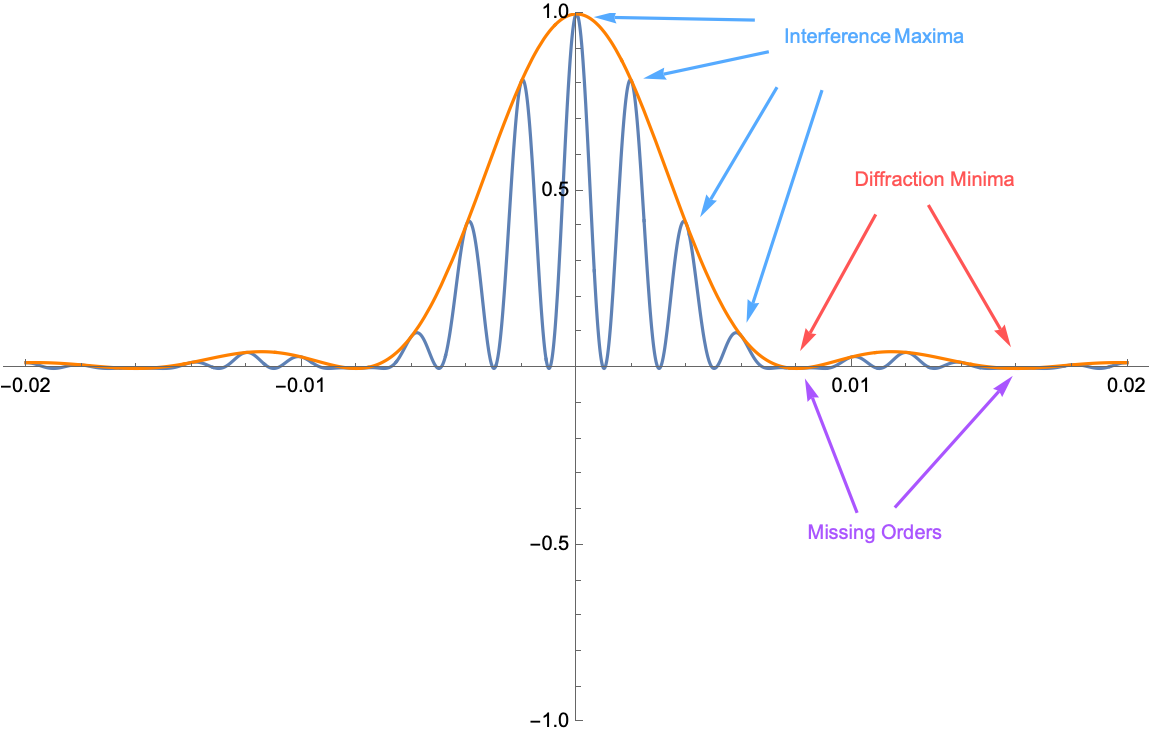
\includegraphics[scale=0.7]{plot.png}
            \end{center}

            Here the envelope is in orange, and the interference pattern is in blue. We can see that there are interference maxima occur at $y = 0, \pm 0.002, \pm 0.006$ and so on. Similarly, the diffraction minima is the minimum of the envelope, which is at $y = \pm 0.008, \pm 0.016$ and so on. The missing orders are where the diffraction minima and interference maxima coincide, so at $\pm 0.08, \pm 0.016$, etc.



        \end{solution}
    \end{enumerate}
\end{document}